%% LyX 1.5.2 created this file.  For more info, see http://www.lyx.org/.
%% Do not edit unless you really know what you are doing.
\documentclass[english]{bioinfo}
\usepackage[latin1]{inputenc}
\usepackage{subfigure}
\setcounter{secnumdepth}{3}
\setcounter{tocdepth}{3}
\usepackage{esint}
\IfFileExists{url.sty}{\usepackage{url}}
                      {\newcommand{\url}{\texttt}}

\makeatletter
%%%%%%%%%%%%%%%%%%%%%%%%%%%%%% Textclass specific LaTeX commands.
 \usepackage{amsmath}
 \usepackage{amsfonts}
 \usepackage{natbib}
 \usepackage{ae}

%%%%%%%%%%%%%%%%%%%%%%%%%%%%%% User specified LaTeX commands.
\usepackage{crop}
\copyrightyear{2008}
\pubyear{2008}

\usepackage{babel}
\makeatother

\begin{document}
\selectlanguage{english}
\firstpage{1}

\title {A Gaussian Process Toolkit for Inference of Latent Chemical Species with Appplications in Inferring Transcription Factor Activities}

\author {Pei Gao\,$^{1}$, Antti Honkela\,$^{2}$, Magnus Rattray\,$^{1}$
and Neil D. Lawrence\,$^{1,*}$%
\thanks {to whom correspondence should be addressed} }

\address {$^{1}$School of Computer Science, University of Manchester, Kilburn Building, Oxford Road, Manchester, M13 9PL\\
$^{2}$Department of XXXXXXXX, Address XXXX etc.}
\history {Received on XXXXX; revised on XXXXX; accepted on XXXXX}

\editor {Associate Editor: XXXXXXX}
\maketitle

\begin{abstract}

\section{Motivation:}

Inference of \emph{latent chemical species} in biochemical interaction
networks is a key problem in estimation of the structure and parameters
of the genetic, metabolic and protein interaction networks that underpin
all biological processes. We present a framework for Bayesian marginalisation
of these latent chemical species through Gaussian process priors. 

\section{Results:}

We apply our approach to three different biological data sets. We
focus on the problem of inference of transcription activity and consider
signaling and developmental networks. 

\section{Availability:}

The software and data for recreating all the experiments in this paper
is available in MATLAB from \url{http://www.cs.man.ac.uk/~neill/gpsim} 

\section{Contact:}

\url{neill@cs.man.ac.uk}
\end{abstract}


\textbf{\emph{Magnus pointed out that what we do is not just useful
for latent functions, but also in the case where the system isn't
closed loop. A closed loop system defines the type of function involved
at each point, an open system (such as we look at) doesn't. So even
if we had observations for all functions involved we would still need
our GP priors for continuity. Need to embed this somewhere.}}


\section{Introduction}

The use of ordinary differential equations to model biological subsystems
is already a well established approach \cite{}. More
recently attention has turned to methodologies for fitting the parameters
of these equations in the context of a particular experiment or set
of experiments \cite{}.

Ordinary differential equations (ODE) are an approximation to the
underlying chemical master equation. In an ODE the intrinsic variability
in the reactants is ignored. However, this variability becomes less
significant as the size of the system increases. Since most biological
experiments cannot isolate expression levels in a single cell we are
generally viewing data that is collated from a significant number
of cells. Therefore, for many experiments of interest we consider
the assumptions behind the approximation to be broadly valid. 

Significant progress has been made on parameter estimation in the
context of differential equations and through the use of advanced
Monte Carlo techniques it is even possible to, given a specific data
set, rank model structures through the use of Bayes factors
\citealp{Vyshemirsky:ranking08}.  This shows the potential for these
techniques to be closely integrated with biological investigations,
informing the process of biological experimental design.

A remaining problem for these approaches is dealing with the case
where one or more of the chemical species in the system are unobserved.
This is a common problem, it is a natural consequence of the fact
that some quantities are relatively easy to measure in a high throughput
manner (\emph{e.g.} mRNA concentrations with microarray), whereas
others are much more difficult to measure on a large scale (\emph{e.g.}
protein concentrations such as transcription factors). In this paper
we advocate the use of Gaussian processes to define prior distributions
over these \emph{latent chemical species}. This allows us to marginalise
their contributions in the interaction network of interest. We present
a basic toolkit of algorithms based on Gaussian processes which allow
us to consider different response models (Michaelis Menten kinetics,
repression responses) and cascades of interactions in which chemical
species of interest are missing. The application domain we consider
is inference of transcription factor (TF) activity in both developmental
and signalling networks. Inference of TF activity in a given network
is a well studied problem with both genome wide approaches (\emph{e.g.}
\citealp{Liao:nca03,Sanguinetti:chipdyno06,Sanguinetti:chipvar06})
and algorithms designed for a sub set of genes (\emph{e.g.} \citealp{Nachman:inferring04,Rogers:model06b,Khanin:repression06,Barenco:ranked06}).
Our approach is most directly inspired by \cite{Barenco:ranked06}
who infer transcription factor activity in a single input module network
motif through a differential equation with a linear response. We build
on their work to consider simple cascade networks and non-linear response
models such as Michaelis Menten kinetics and repression responses
(\citealp{Alon:systems06,Khanin:repression06}).

Gaussian processes \cite{Rasmussen:book06} are probabilistic models
of functions that encode particular assumptions about the function
such as smoothness and timescale. They are commonly applied in the
context of regression and interpolation. An attractive characteristic
of the Gaussian process (GP) is that the result of any linear operator
on the function leads to another GP, we will exploit this when applying
GPs in the context of differential equations. 

Our focus in this paper will be the inference of transcription factor
activities given mRNA concentrations. We start by considering the
model given in \cite{Barenco:ranked06} and reviewing the work done
by \cite{Lawrence:transcriptionalGP06} who provided the first
treatment of this model with Gaussian processes. Then, in
Section~\ref{sub:repressionModel}, we extend our model to the case of
repression. We follow \cite{Khanin:repression06} and apply the
model in the context of the SOS system where genes are controlled by
the transcriptional repressor protein LexA. In both these cases, no
model of transcription factor translation is included. In our final
example (Section~\ref{sub:cascadedDifferentialEquations}) we show how,
in the context of \emph{Drosophila mesoderm} development a model of
translation can be incorporated to improve the quality of the
transcription factor inference.


\section{Methods and Results}

Consider the following simple model of gene regulation proposed by
\cite{Barenco:ranked06}, \[
\frac{\mathrm{d}x_{j}\left(t\right)}{\mathrm{d}t}=B_{j}+S_{j}f\left(t\right)-D_{j}x_{j}\left(t\right),\]
here the changing level of a gene $j$'s expression,
$x_{j}\left(t\right)$, is given by a combination of a basal
transctiption rate, $B_{j}$, a sensitivity, $S_{j}$, to its governing
TF's activity, $f\left(t\right)$, and the decay rate of the mRNA,
$D_{j}$. The differential equation can be solved for
$x_{j}\left(t\right)$ giving
%
\begin{equation}
x_{j}\left(t\right)=\frac{B_{j}}{D_{j}}+S_{i}\int_{0}^{t}e^{-D_{i}\left(t-u\right)}f\left(u\right)\mathrm{d}u,\label{eq:linearSolution}
\end{equation}
%
where we have ignored any transient terms.

Our general approach is to assume that $f\left(t\right)$ was drawn
from a Gaussian process. A Gaussian process (GP) is a prior
distribution over functions that leads to highly flexible non-linear
functions in which characteristics such as the stationarity, the
roughness and the timescale of the signal can be controlled. Gaussian
processes are the functional analogue of the Gaussian distribution,
they are fully specified by a mean function, $\mu\left(t\right)$, and
a covariance function, $k\left(t,t^{\prime}\right)$. The mean function
is an unconstrained function of time, whilst the covariance function
is constrained to be a positive definite function. Various covariance
functions can be used, we will predominantly make use of the squared
exponential covariance (sometimes known as the Gaussian or RBF
covariance),
%
\[
k\left(t,t^{\prime}\right)=e^{-\frac{\left(t-t^{\prime}\right)^{2}}{l^{2}}}.\]
%
An important characteristic of a GP is that any linear operation
applied to the function drawn from a GP leads to a function that is
drawn from a related GP. This is the functional analogue of linear
operations applied to samples from a Gaussian distribution. We note
that (\ref{eq:linearSolution}) is a linear operation on
$f\left(t\right)$: it only involves integrals sums and products
applied to $f\left(t\right)$. The properties of GP tell us that if
$f\left(t\right)$ was drawn from a GP with covariance function
$k_{f,f}\left(t,t^{\prime}\right)$ then $x_{j}\left(t\right)$ will
also be drawn from a GP with a covariance function given by
\[
k_{x_{j},x_{j}}\left(t,t^{\prime}\right)=S_{j}^{2}\int_{0}^{t}e^{-D_{j}\left(t-u\right)}\int_{0}^{t^{\prime}}e^{-D_{j}\left(t^{\prime}-u^{\prime}\right)}k_{f,f}\left(t,t^{\prime}\right)\mathrm{d}u^{\prime}\mathrm{d}u.
\]
Furthermore, the cross covariances between the $f\left(t\right)$ and
$x_{j}\left(t\right)$ will be given by
\[
k_{x_{j},f}\left(t,t^{\prime}\right)=\int_{0}^{t}e^{-D_{i}\left(t-u\right)}k_{f,f}\left(t,t^{\prime}\right)\mathrm{d}u.
\]
Finally, if our data consist of several genes, $\left\{
x_{j}\left(t\right)\right\} _{j=1}^{N}$, cross covariances between the
genes can be computed, 
\[
k_{x_{i},x_{j}}\left(t,t^{\prime}\right)=S_{i}S_{j}\int_{0}^{t}e^{-D_{i}\left(t-u\right)}\int_{0}^{t^{\prime}}e^{-D_{j}\left(t^{\prime}-u^{\prime}\right)}k_{f,f}\left(t,t^{\prime}\right)\mathrm{d}u^{\prime}\mathrm{d}u.
\]
The basal transcription rate then appears in the mean function to
define the mean of the Gaussian process for $x_{j}\left(t\right)$ as a
constant $\frac{B_{j}}{D_{j}}$.

As was shown in \cite{Lawrence:transcriptionalGP06}, if
$f\left(t\right)$ is drawn from a GP with a squared exponential
covariance function, we can analytically define a probabilistic model
of the expression data for which the parameters of the differential
equation, $B_{j},\, S_{j},\, D_{j}$ and the timescale $l$ can all be
determined, either through maximum likelihood or Bayesian sampling. We
illustrate this by repeating their results here.


\subsection{p53 Activity}

The transcription factor p53 is a tumour repressor which is generally
known as a transcription factor activated during DNA damege. According
to \cite{Barenco:ranked06}, irradation is performed to disrupt the
equilibrium of the p53 network and the transcription of p53 target
genes are then stimulated. Seven samples of the expression levels of
the target genes in three replicas are collected as the raw time
course data. 

\subsubsection{Linear Model}

In this section we recreate the results presented by
\citeauthor{Lawrence:transcriptionalGP06} for the linear model with
several key differences. Firstly, in the original paper
\citeauthor{Barenco:ranked06} constrained $f\left(0\right)$ to be
zero, forcing the basal transcription rate to account for all
transcription at time $t=0$. This constraint was not included in
\citeauthor{Lawrence:transcriptionalGP06} but is included here. This
allows us to incorporate the prior information of the latent TF
profiles as much as possible and Secondly,
\citeauthor{Lawrence:transcriptionalGP06} used an unormalised version
of the Affymetrix array data. We found that simple median based
normalisation removed the effect of a couple of repeats that were
anomalously high.  Inspection of the processed data used by
\citeauthor{Barenco:ranked06} showed that they had also dealt with
these anomalies so here we considered the normalised array data.

\begin{figure*}[t]
\centering
\subfigure{
	\label{fig:activation:a}
	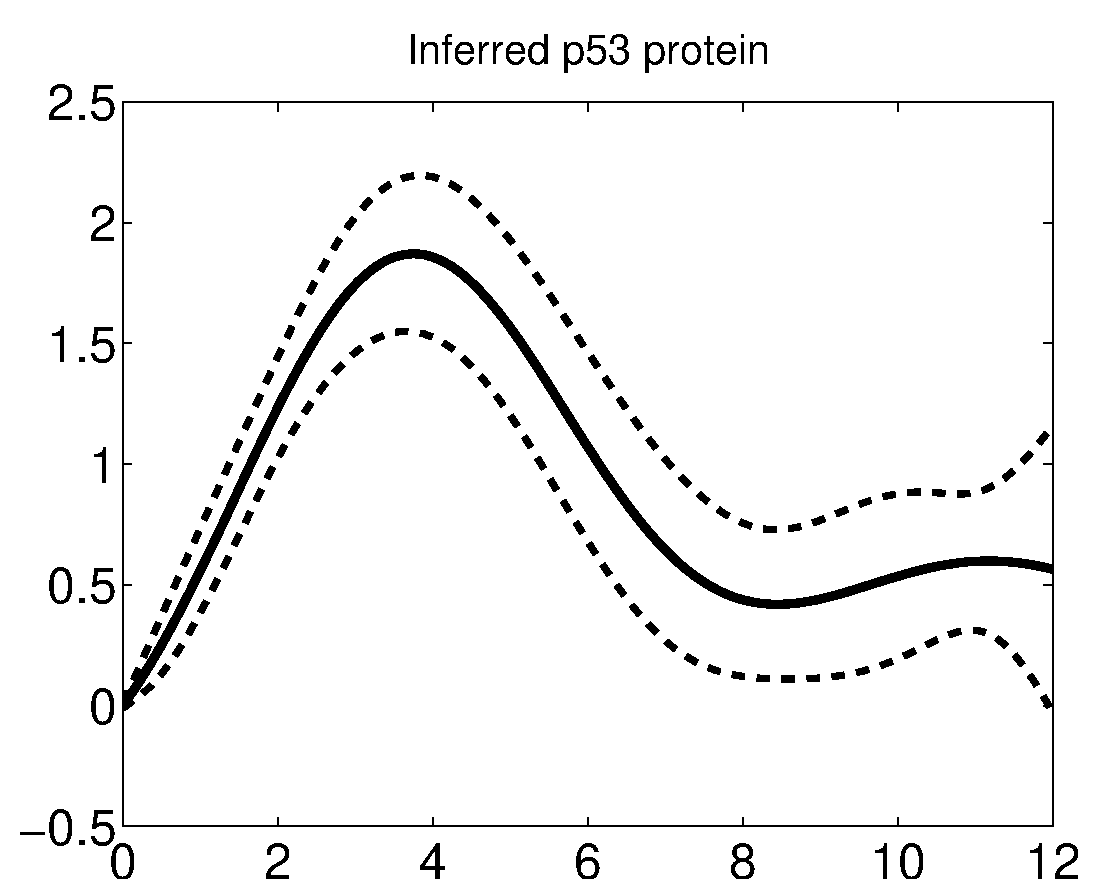
\includegraphics [height=1.6in, width=0.3\textwidth] {results/RBFLinear/demBarenco1_profile2.eps} }
\subfigure{
	\label{fig:activation:b} 
	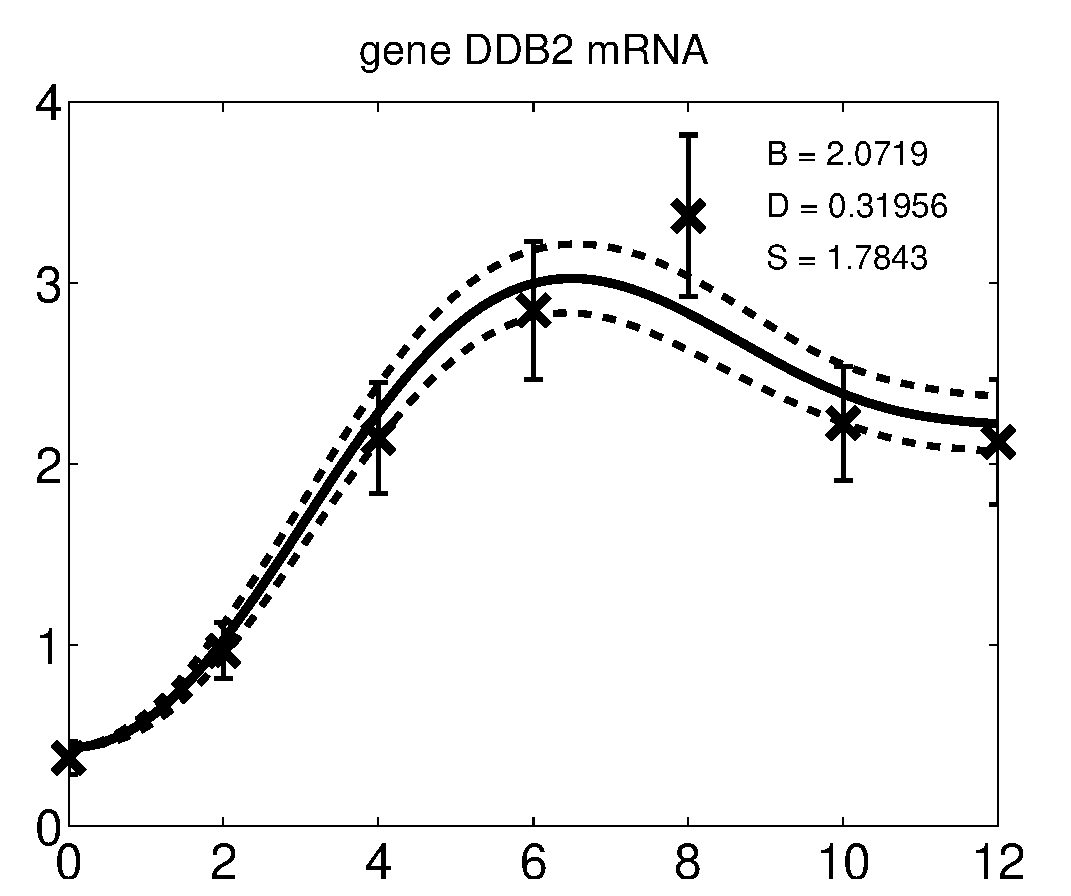
\includegraphics [height=1.6in, width=0.3\textwidth]{results/RBFLinear/demBarenco1_ExprsProfile_Rep2_Gene1.eps} }
\subfigure{
	\label{fig:activation:c}
	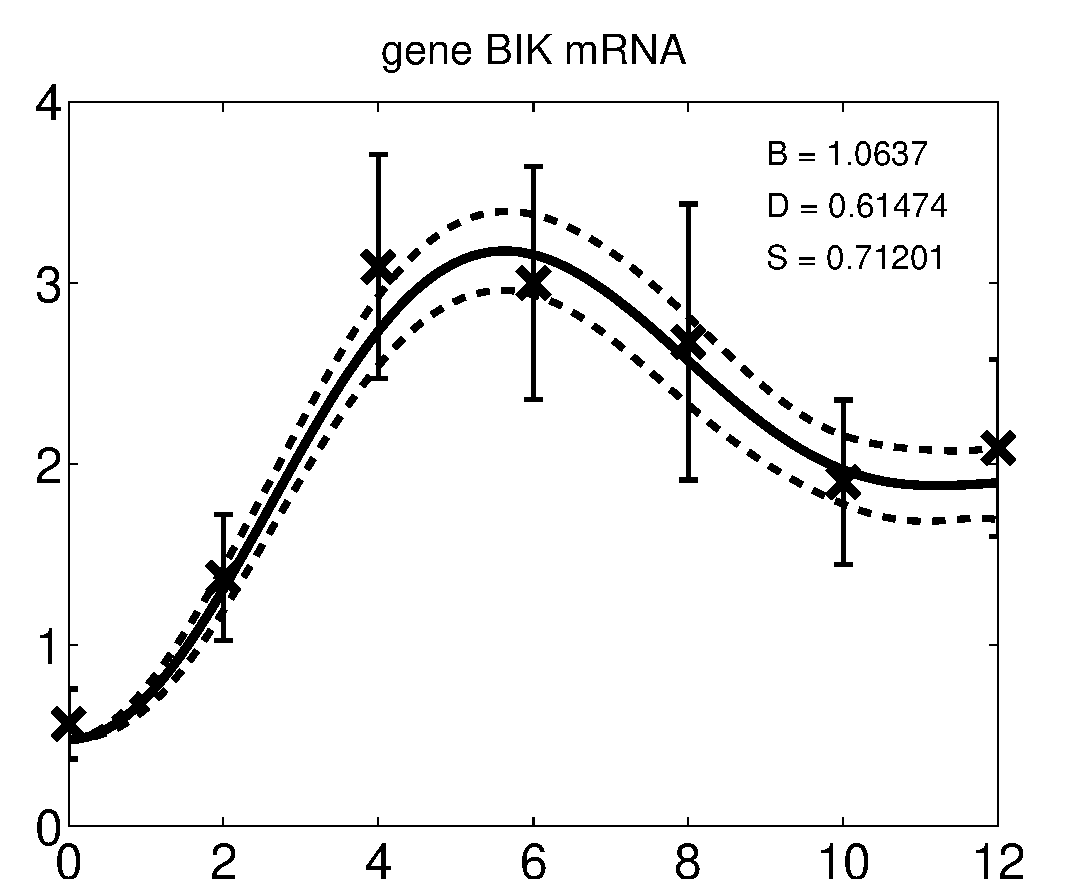
\includegraphics [height=1.6in, width=0.3\textwidth]{results/RBFLinear/demBarenco1_ExprsProfile_Rep2_Gene2.eps} }
\subfigure{
	\label{fig:activation:d}
	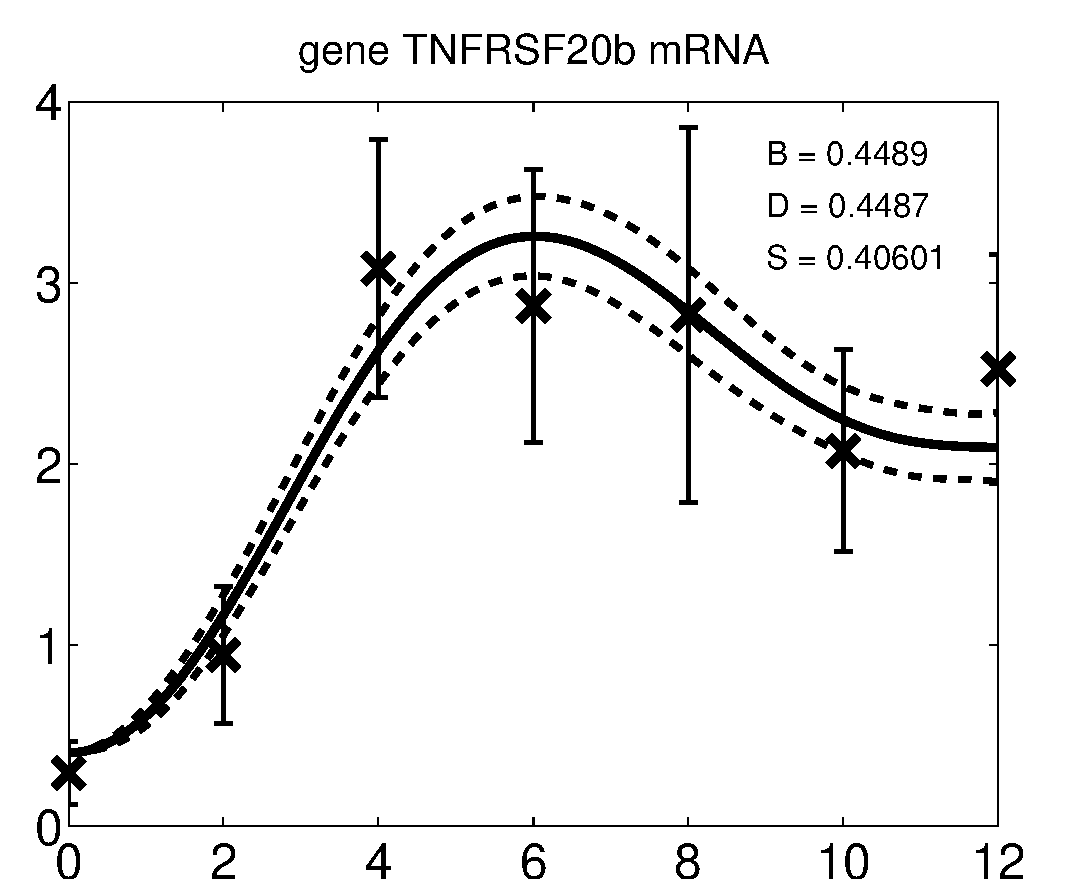
\includegraphics [height=1.6in, width=0.3\textwidth]{results/RBFLinear/demBarenco1_ExprsProfile_Rep2_Gene3.eps} }
\subfigure{
	\label{fig:activation:e}
	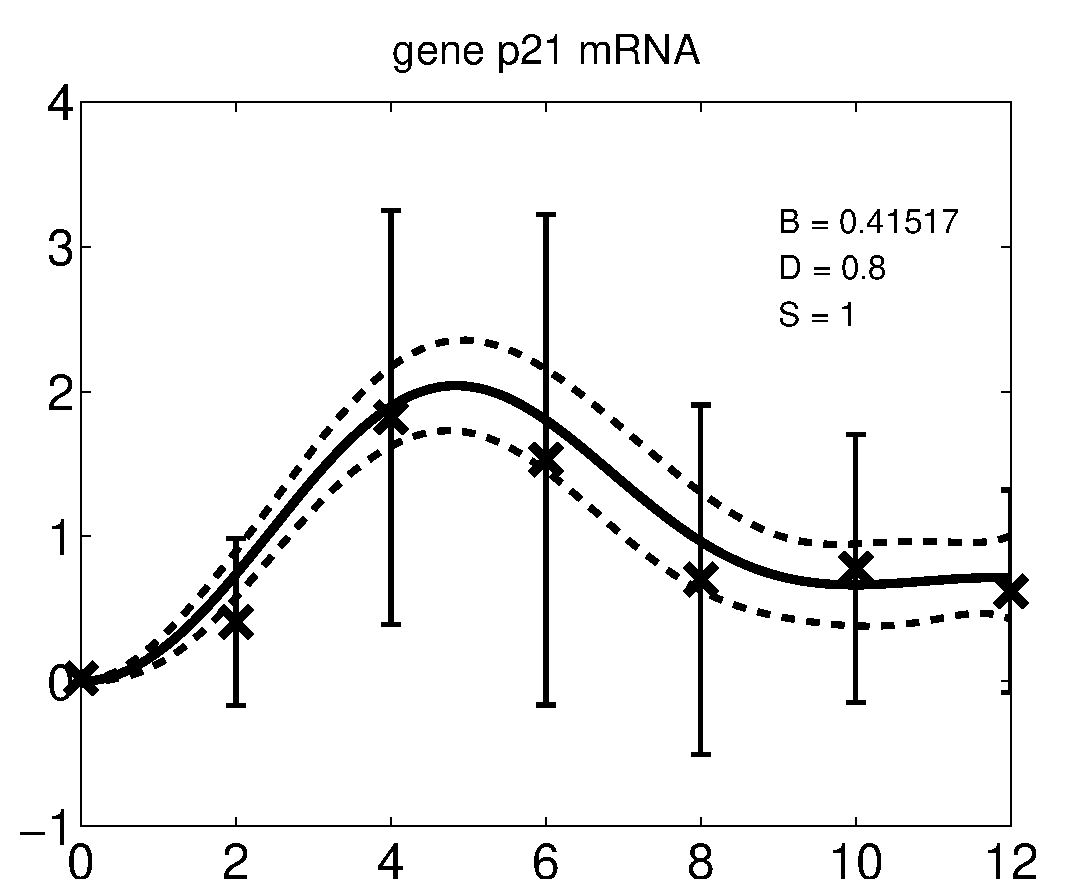
\includegraphics [height=1.6in, width=0.3\textwidth] {results/RBFLinear/demBarenco1_ExprsProfile_Rep2_Gene4.eps} }
\subfigure{
	\label{fig:activation:f}
	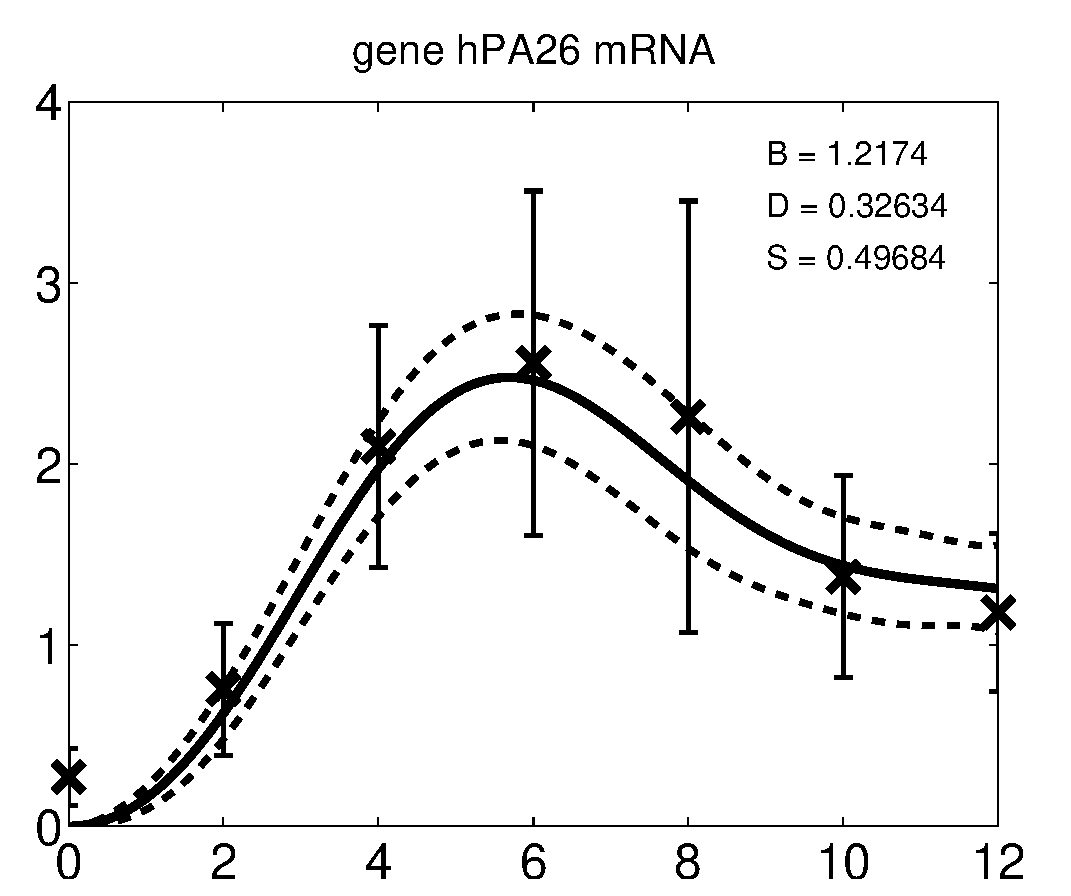
\includegraphics [height=1.6in, width=0.3\textwidth] {results/RBFLinear/demBarenco1_ExprsProfile_Rep2_Gene5.eps}
}
\caption{Results for p53 using the linear model and a GP with RBF
  kernel: (a) predicted protein concentration; (b) predicted
  expression level for DDB2; (c) predicted expression level for BIK;
  (d) predicted expression level for TNFRSP20b; (e) predicted
  expression level for p21; (f) predicted expression level for
  hPA26. Solid lines represent the mean inference, dashed lines are
  95\% credibility intervals, and the crosses are the observed gene
  expression data.} \label{fig:activation}
\end{figure*}


In Figure \ref{fig:activation} we show results of the TF inference as
well as the model parameter estimations. The latent TF activity
profiles are reconstructed with 95\% confidence bounds. It can be seen
that it resembles the activity profile of p53 meansured by Western
blot \citeauthor{Barenco:ranked06}. The kinetic parameters in the
model are also shown to be closely matched with the results from
\citeauthor{Barenco:ranked06}.



\subsubsection{MAP Laplace Approximation}

The differential equation with a linear response is an attractive
model to use in the context of GPs as it allows the joint distribution
over the gene expression and TF activity to be determined
analytically, given the model parameters. However, as a model, it has
some shortcomings.  Firstly, it treats both the gene expression and
the TF activity as GPs. Since a GP cannot encode the information that
a function is constrained positive, this means that the concentrations
are \emph{a priori} allowed to be negative. Whilst the posteriors, in
the region where there is data, tend to stay positive (see
Figure~\ref{fig:activation} ), when the predictions move away from the
data they allow the TF activity to become negative.  A potential
solution to this problem is to place a GP prior over, for example, the
log concentration of the TF activity. However, this, in effect, is a
non-linear response in the differential equation. The non-linear
response means that it is no longer possible to construct the joint
distribution over gene expression and TF activity in a closed form.
We must, necessarily, turn to approximations to make progress. In
\cite{Lawrence:transcriptionalGP06} the use of a MAP-Laplace
approximation is suggested. They demonstrate how the concentration of
the TF activity can be constrained positive by placing the GP in log
space.

Consider the following modification to the model, 
\[
\frac{\mathrm{d}x_{j}\left(t\right)}{\mathrm{d}t}=B_{j}+S_{j}g\left(f\left(t\right)\right)-D_{j}x_{j}\left(t\right),
\]
where $g\left(\cdot\right)$ is a non-linear function. The differential
equation can still be solved, 
%
\begin{equation}
x_{j}\left(t\right)=\frac{B_{j}}{D_{j}}+S_{i}\int_{0}^{t}e^{-D_{i}\left(t-u\right)}g\left(f\left(u\right)\right)\mathrm{d}u,\label{eq:linearSolution}
\end{equation}
%
but there is now a non-linear operation on $f\left(t\right)$ before
the product and integral. The gene expression level is therefore no
longer a GP. The MAP-Laplace approach involves finding a maximum
\emph{a posteriori} estimate for the function $f\left(t\right)$ and
making a second order Taylor approximation at that point to the log
likelihood.  This approximation is itself a Gaussian process and leads
to an approximation to the marginal likelihood
\cite{Rasmussen:book06}. Derivatives can then be taken with respect
to the model parameters and the approximation maximised. The
MAP-Laplace's approximation becomes exact in the case where
$g\left(\cdot\right)$ is \emph{linear}. This is also useful in
practice, as well as providing a sanity check that the solutions are
consistent, the MAP-Laplace approach is unconstrained in the choice of
covariance function for $f\left(t\right)$. Naive implementation of the
linear response model for a general covariance function would require,
in general, numerical evaluation of the double integrals in () and
(). The use of the MAP-Laplace approach involves only a single
numerical integral. Results of inferring p53 TFA using MAP-Laplace
with the linear model are shown in Figure~\ref{TFbyMLPLinear} and
\ref{ParamsbyMLPLinear}. As can be seen, a GP with a MLP kernel with
MAP-Laplace algorithm is able to provide even better performance on
the inference. The use of MLP kernel may help avoid the unnecessary
fluctuation caused by the nature of the RBF kernel.

In this paper we build on the work of
\cite{Lawrence:transcriptionalGP06} in two major ways. We go beyond
the simple exponential response model considered exploring a
Michaelis-Menten kinetics inspired response and a response that has
been suggested as appropriate for repression
\cite{Alon:systems06}. We also extend the algorithm to learn the
parameters of the differential equation by maximising the
approximation to the log likelihood.


\subsubsection{Michaelis Menten Kinetics}

Michaelis Menten kinetics reaction kinetics were designed for the case
where a chemical reaction is enabled through an enzyme. If the
concentration of the enzyme is much lower than the concentration of
the substrate the reaction rate becomes limited by the reduced enzyme
availability. The justification in the context of modelling
transcription is that the reaction is that there are a limited number
of binding sites on the genome for the transcription factor. This
`bottle neck' has the same effect as a reduced availability of enzyme
and Michaelis Menten kinetics are therefore preferred as a model of
transcription.

We implemented Michaelis Menten kinetics for the p53 data by taking
the non-linearity to have the following form
\[
g_i\left(f\left(t\right)\right)=\frac{e^{f\left(t\right)}}{\gamma_i + e^{f\left(t\right)}},
\]
where the Michaelis constant for the $i$th gene is given by $\gamma_i$ and we are using $f\left(t\right)$ to model the log of the TF activity.

\textbf{Experimental Set up and results}

\subsection{Repression\label{sub:repressionModel}}

\textbf{DESCRIPTION OF REPRESSION PROBLEM AND RESULTS}


\subsection{Cascaded Differential Equations\label{sub:cascadedDifferentialEquations}}

As a final example we consider a simple cascade of differential equations.
Returning to the framework of the linear model we
consider the case where the TF activity is determined by its own mRNA.
In other words we model the process of translation from mRNA to protein
for the TF. The simple model we consider would only be appropriate
in the case where the TF does not require activation after translation,
for example by phosphorolation. The model is, therefore, not appropriate
for many signalling pathways, but seems sensible in the context of
development where TFs typically can act directly after translation.
We therefore considered an example of the development of the mesoderm
in \emph{Drosophila Melanogaster}.

{\bf {\em Wasn't this model inspired by something you read magnus? Need to mention that here.}}

We take the production rate of active transcription factor to be given by,
\[
\frac{\mathrm{d}f\left(t\right)}{\mathrm{d}t}=\sigma y\left(t\right) - \delta f\left(t\right),
\]
where $\delta$ gives the decay rate of the active TF and $\sigma$
gives a rate of transcription and $y\left(t\right)$ is the concentration of the
transcription factor's mRNA concentration.
 
If we assume that $y\left(t\right)$ was drawn from a GP with the squared
exponential covariance function, then $f\left(t\right)$ is also a GP that is
governed by a special case of the covariance function derived in
(\ref{eq:simKernel}),
%
\textbf{SHOW EQUATION RESULT HERE}
%
This gives us a new covariance function governing $f\left(t\right)$. It turns out
that we can use this prior over $f\left(t\right)$ in the model given in (\ref{})
and derive the associated prior distribution for the target genes of
the TF, $\left\{x_{j}\left(t\right)\right\}_{j=1}^N$. The derivation and form of
the resulting covariance function are rather involved and have been
relegated to the supplementary material.

We applied the driven input model to a simple cascade in
\emph{Drosophila mesoderm} development. We focussed on the
transcription factor Mef2 (Myocyte enhancing factor 2). We identified
six targets of Mef2 through Chromatin immunoprecipitation assays
provided by \textbf{reference Eileen's data here}. We reconstructed
the transcription factor activity of Mef2 ...

\textbf{Pei will try and produce similar results with no driven input here ...}.
\textbf{CASCADE RESULTS GO HERE}
\begin{figure*}[t]
\centering
\subfigure{
	\label{fig:gpdisim:a}
	\includegraphics[height=2.5in] {ISMBMef2/demMef2Dros4_ExprsProfile_Gene1.eps} 	}
\subfigure{
	\label{fig:gpdisim:b}
	\includegraphics[height=2.5in] {ISMBMef2/demMef2Dros4TF_profile.eps} }
\subfigure{
	\label{fig:gpdisim:c}
	\includegraphics[height=2.5in] {ISMBMef2/demMef2Dros4_ExprsProfile_Gene2.eps} }
\subfigure{
	\label{fig:gpdisim:d}
	\includegraphics[height=2.5in] {ISMBMef2/demMef2Dros4_ExprsProfile_Gene4.eps} }
\caption{Reconstructed profiles of six genes used for inferrring the Mef2 activity.}
\label{fig:gpdisim}
\end{figure*}

\begin{itemize}
\item Mention that we are aware that this is a short cascade ... reference
Alon for Cascades in developmental networks? pg 90.
\end{itemize}

\section{Discussion}


\section{Conclusion}


\section*{Funding}

This work is funded by BBSRC Grant. No BBS/B/0076X {}``Improved processing
of microarray data with probabilistic models'', EPSRC Grant. No EP/F005687/1
{}``Gaussian Process Models for Systems Identification with Applications
in Systems Biology'' and the EU FP6 Network of Excellence PASCAL.

\section*{Acknowledgement }

For data provision and assistance with our questions we would like
to thank Charles Girardot and Eileen Furlong of EMBL in Heidelberg
(mesoderm development in \emph{D. Melanogaster}), Martino Barenco
and Mike Hubank at the Institute of Child Health in UCL (p53 pathway)
and Raya Khanin and Ernst Wit of the University of Glasgow and the
University of Lancaster (\emph{E. coli} repressor system). 

\bibliographystyle{plainnat}
\bibliography{ismb2008}


\end{document}
